\chapter{Proposed software architecture}
\label{sec:Proposed software architecture}



% \section{Overview}



\section{System architecture choice}
We have chosen to utilise the \textbf{Model-View-Controller} system architecture, separating presentation and interaction from system data. Our clients are the view, the webserver is the controller, and the storage module is the model.

\subsubsection{Advantages}
\begin{itemize}
	\item By keeping the visuals separated from the application data, we can achieve very loose coupling, as well as the ability to easily change the same data from many different views, for example via our desktop and web-based clients. \\
	\item If we ever need to change parts of the program, it will be easy to switch out parts of the code.
\end{itemize}


\subsubsection{Disadvantages}
\begin{itemize}
	\item We will most likely have a larger amount of classes than necessary for a project of this scope. \\
	\item The class hierarchy might become messier, as we will need a larger amount of classes for simple tasks.
\end{itemize}

\section{Design pattern choices}
We will here document the design patterns utilized by the program. We will mention the reasoning behind our choices.

\begin{itemize}
	\item \emph{MVC} (or Model-View-Controller) has not only been utilized on the system as a whole, but also notably in the ASP.net client. By doing this, user interface is clearly separated from the controlling logic of the program, and we get modular code that is easy to maintain and extend.
	\item The \emph{Database Mapper} pattern has been applied when performing transactions between the web server and the database. The system contains a facade exposed to the web server. The facade can be injected with the wanted mapper, which will then connect to the database based on the mapper.
	\item The \emph{Abstract factory} is used in the storage subsystem to create instances of storage. By using this design pattern, we give the subsystem added extendability, simplifying the progress of making plugins that utilize the subsystem.
	\item \emph{bridge pattern} is implemented  in storage is used to easily inject stops.
	\item The \emph{Adapter pattern} has been used when translating alien movie data from other databases to the format used in the main database.
	\item The \emph{Front Controller Pattern} is used when processing requests. Incoming requests is sent through a delegator to the relevant request controller. The controller determines how the request will affect the database. This allows for new request types to be implemented easily.
	\item The \emph{Facade Pattern} is used for each of the subsystems in the program. All subsystems expose a single facade to be accessed by other subsystems, allowing simple communication compared to more complicated communication in which every class could communicate with eachother. Furthermore the pattern allows each subsystem to be self-contained allowing for inner changes to be made frequently as long as the changes does not change the functionality of the facade.
\end{itemize}

\section{Subsystem decomposition}
\label{sec:Subsystem decomposition}
We have grouped our classes into subsystems to create a clearer structure of the program. In this section, we will first show an overview of how the subsystems interact, and then a detailed look at the individual subsystems.\\


\begin{figure}[H]
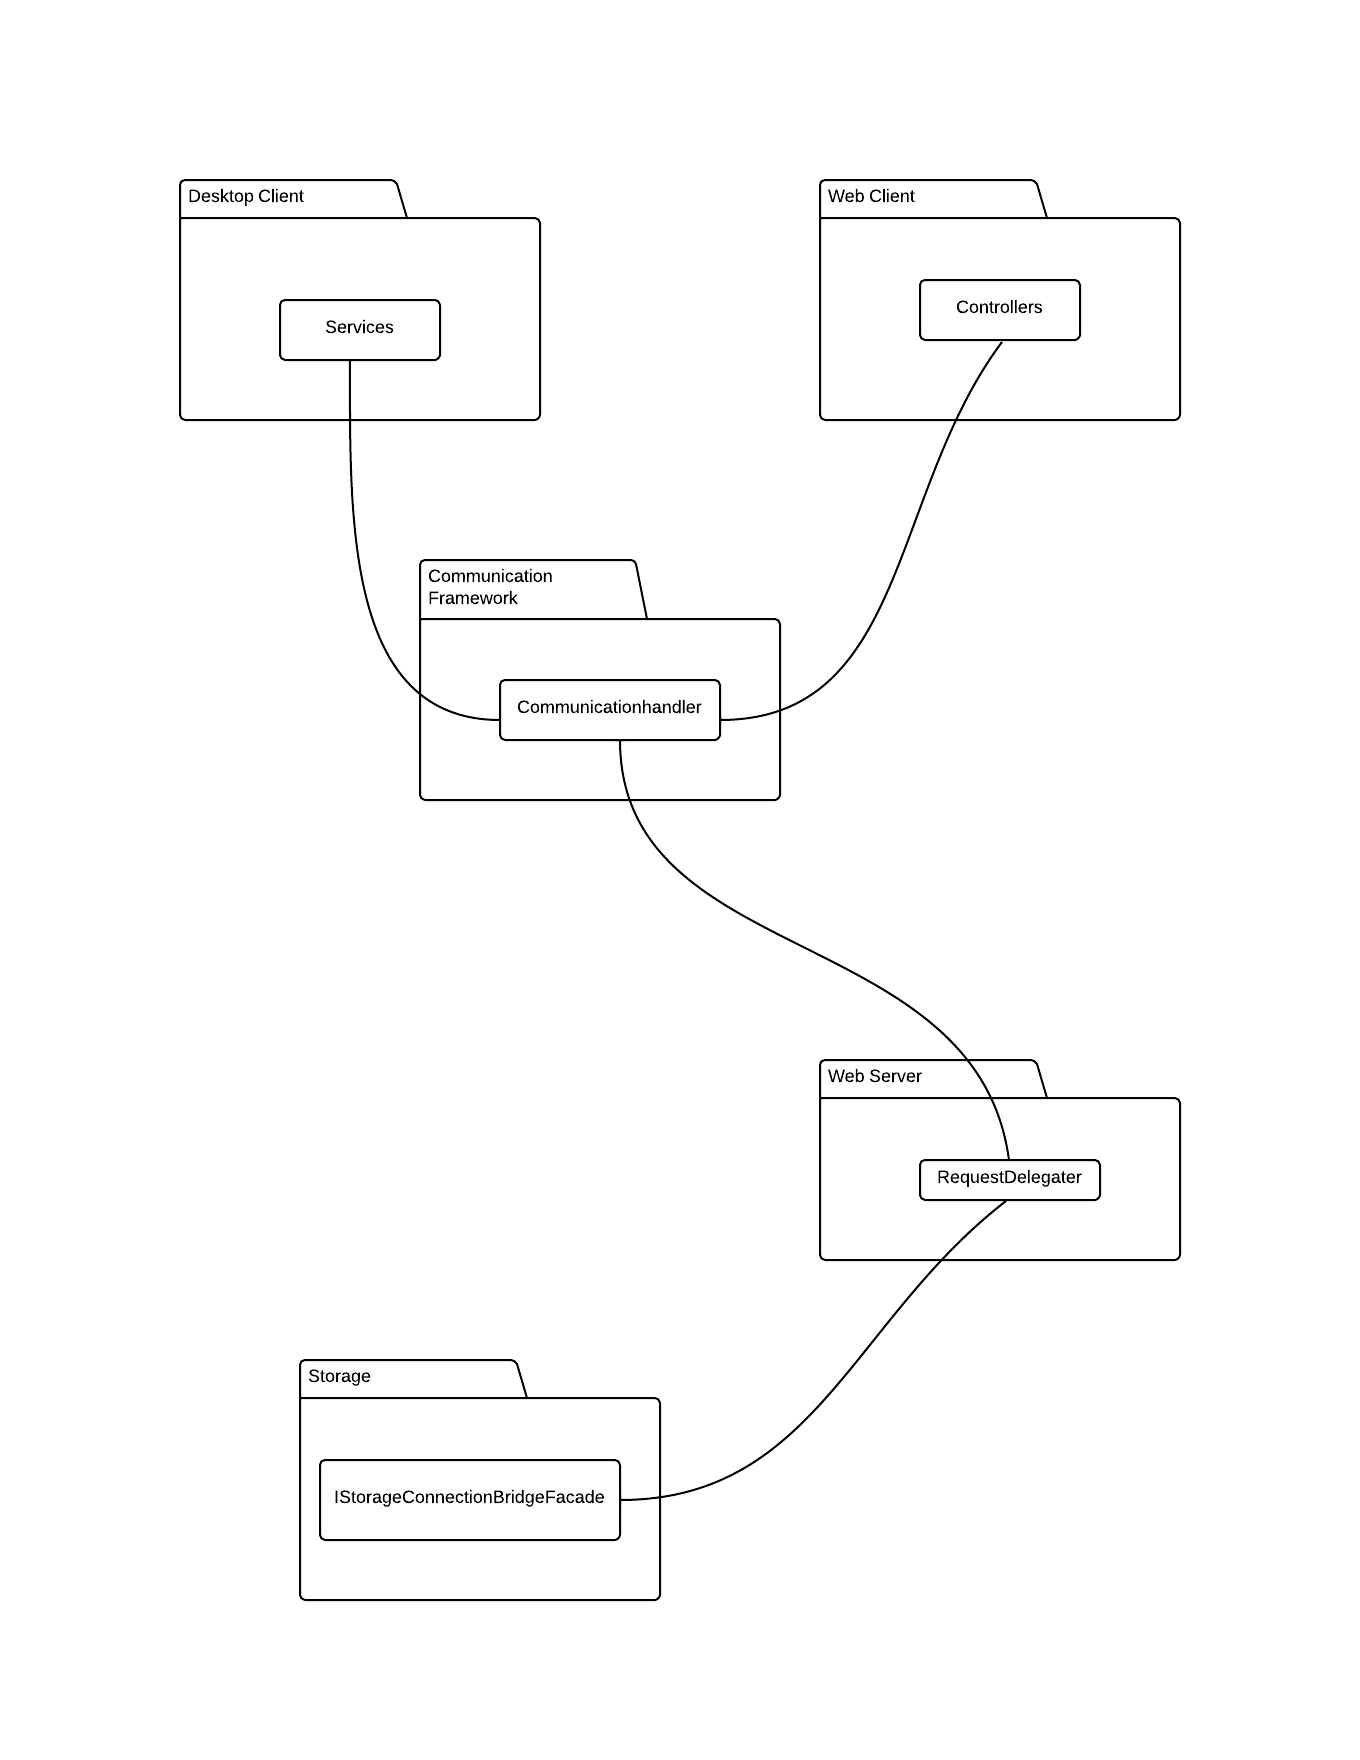
\includegraphics[scale=0.2]{img/FakeIMDbSubsystems.png}
\caption{Fake IMDb Subsystems}
\label{fig:FakeIMDBSubsystems}
\end{figure}

Fake IMDb is divided into five main subsystems with one subsystems for each different clients, communicating with WebServer subsystem through Communication Framework subsystem. WebServer sybsystem use Storage subsystem to get/put data to/from the clients.\\


\begin{figure}[H]
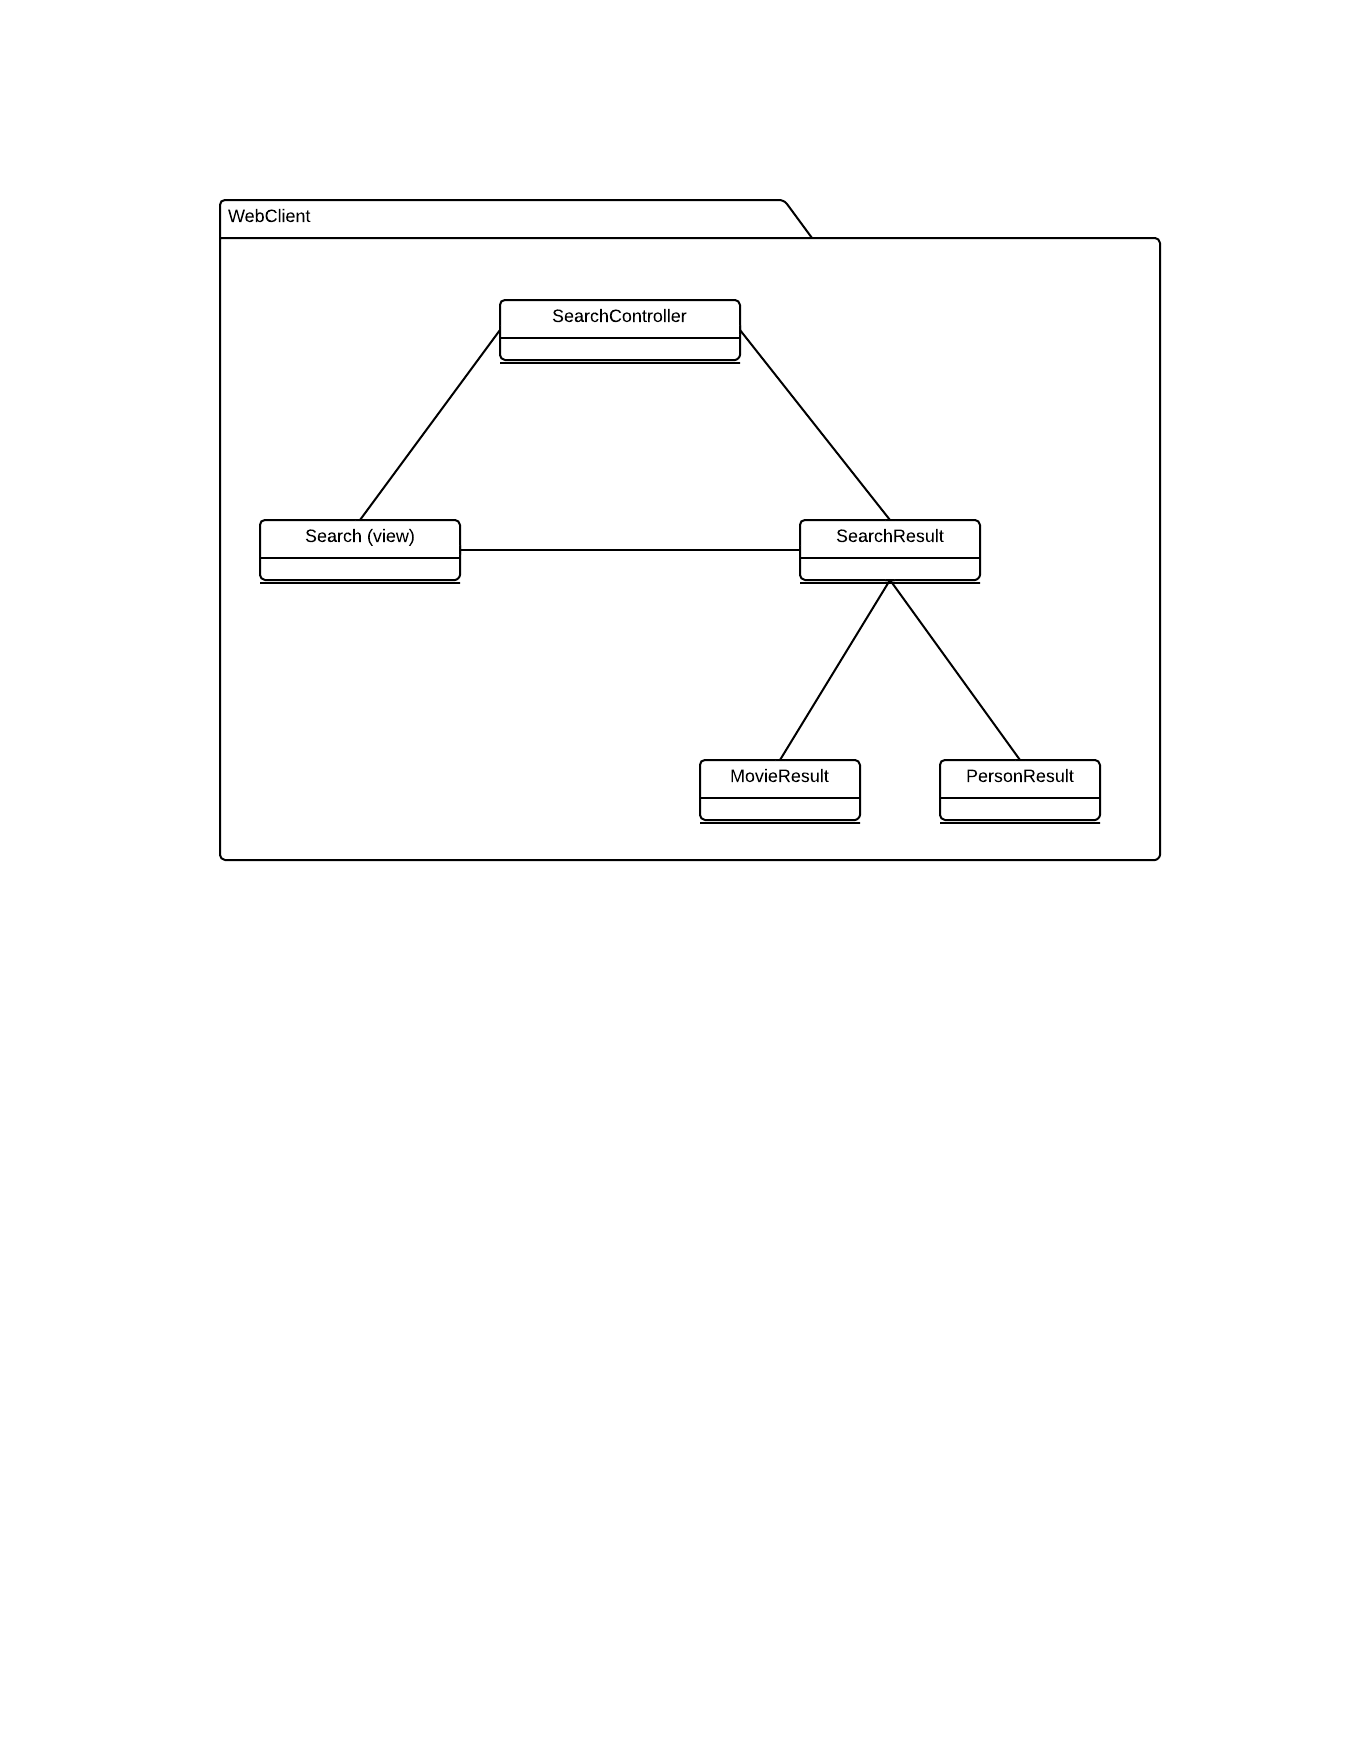
\includegraphics[scale=0.2]{img/WebClientSubsystemSnippet.png}
\caption{A snippet of the Web Client}
\label{fig:WebClientSubsystem}
\end{figure}

The Web Client use ASP.Net framework which have a lot of action going on behind the scene and therefor it will not make sense to show a common static class diagram. Instead  a fraction is shown through a search session. The SearchController use SearchResult to get a movieresult or personresult to show in Search(view)\\



\begin{figure}[H]
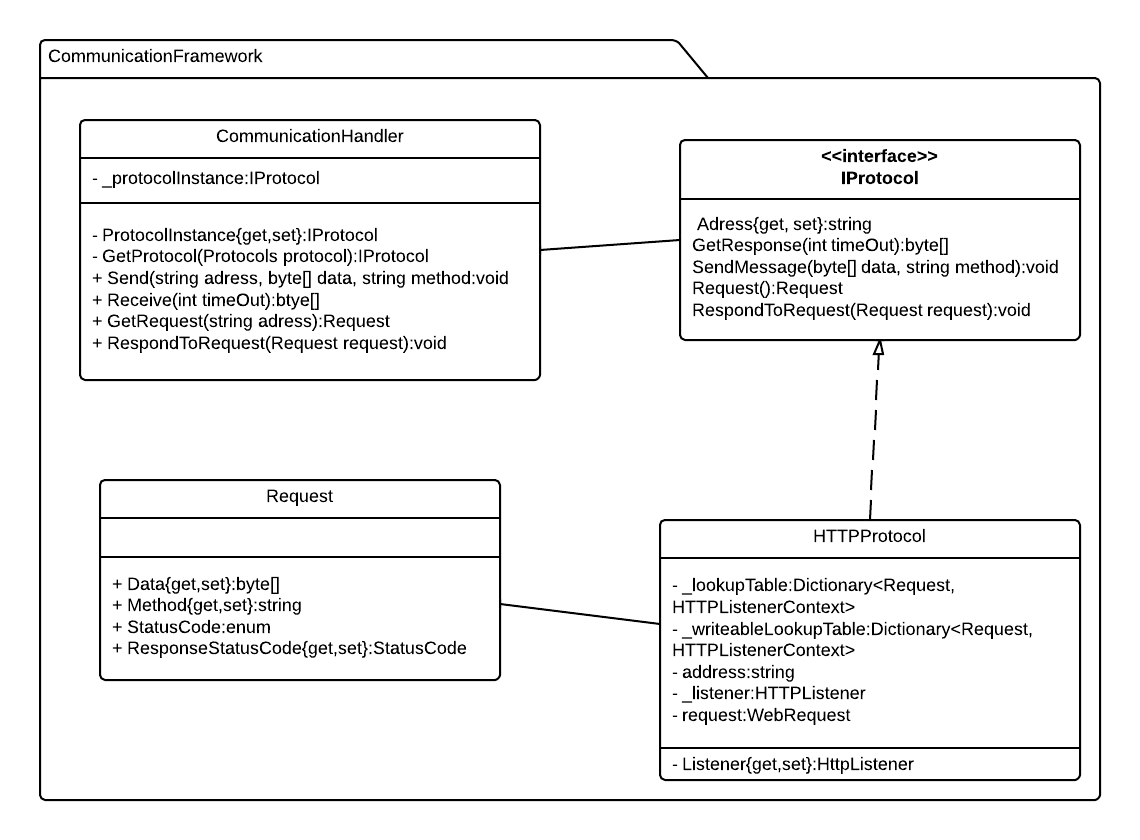
\includegraphics[scale=0.2]{img/CommunicationFrameworkSubsystem.png}
\caption{Communication Framework Subsystem}
\label{fig:CommunicationFramework}
\end{figure}
Here shall be some very wise text about the communication framework subsystem.


\begin{figure}[H]
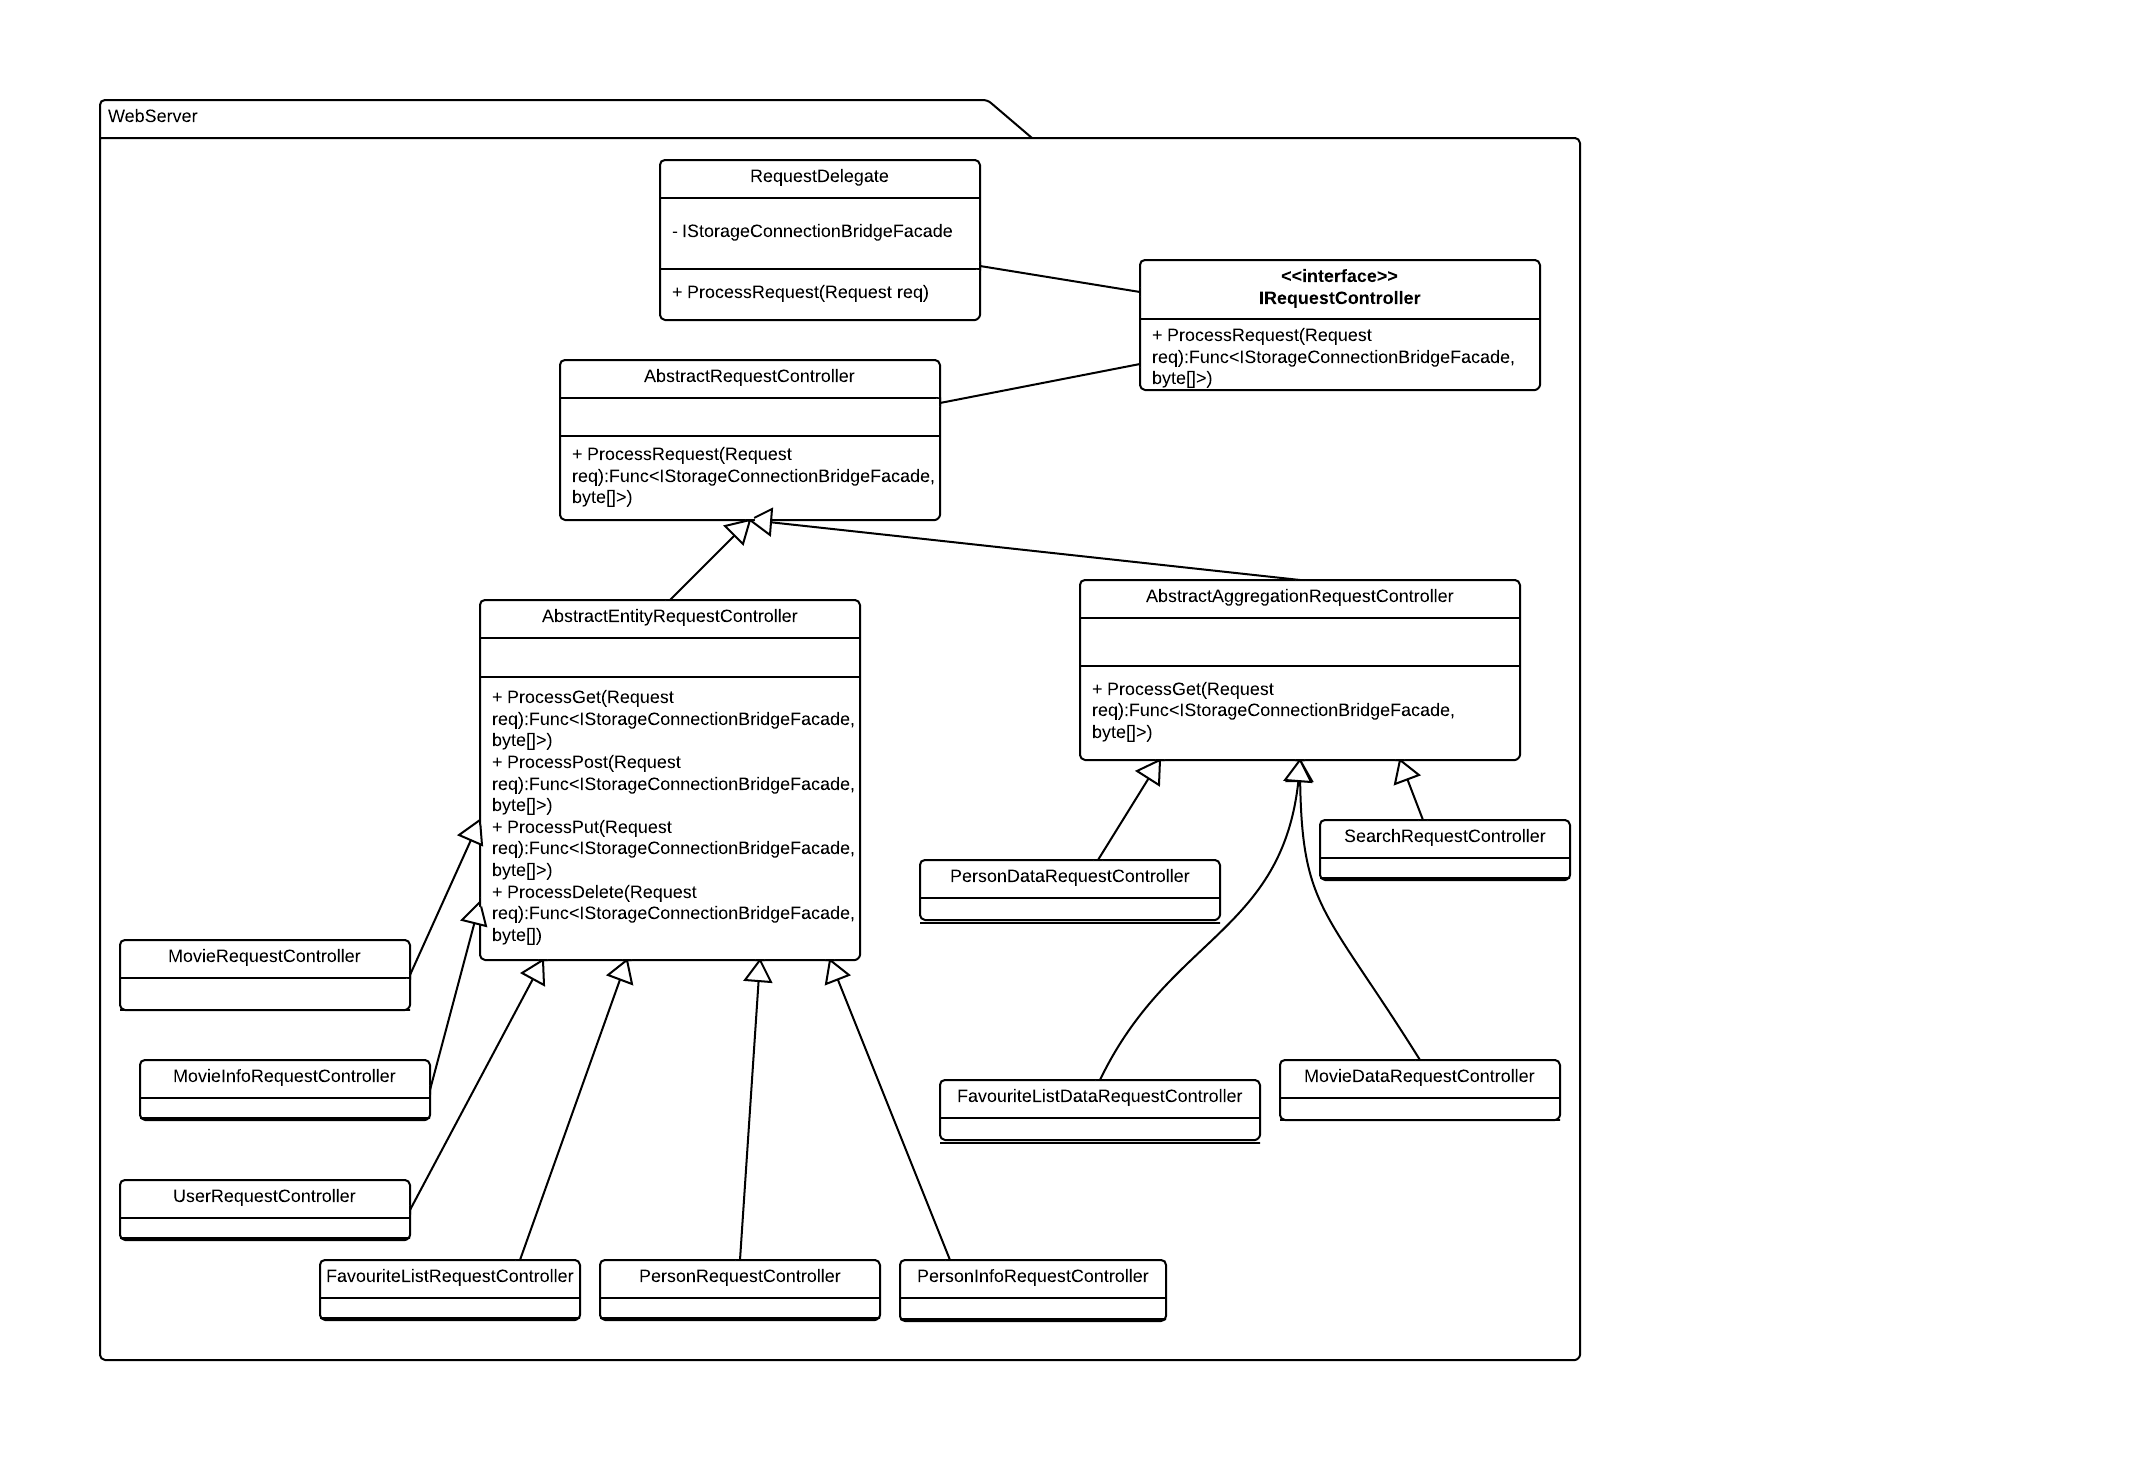
\includegraphics[scale=0.2]{img/NewWebserverSubsystem.png}
\caption{Web Server Subsystem}
\label{fig:WebServer}
\end{figure}

The web server receives a request...

%insert subsystem diagrams here


\section{Hardware/software mapping}
\label{sec:Hardware/software mapping}
Below are the generalized components mapped to hardware or software
\begin{figure}[H]
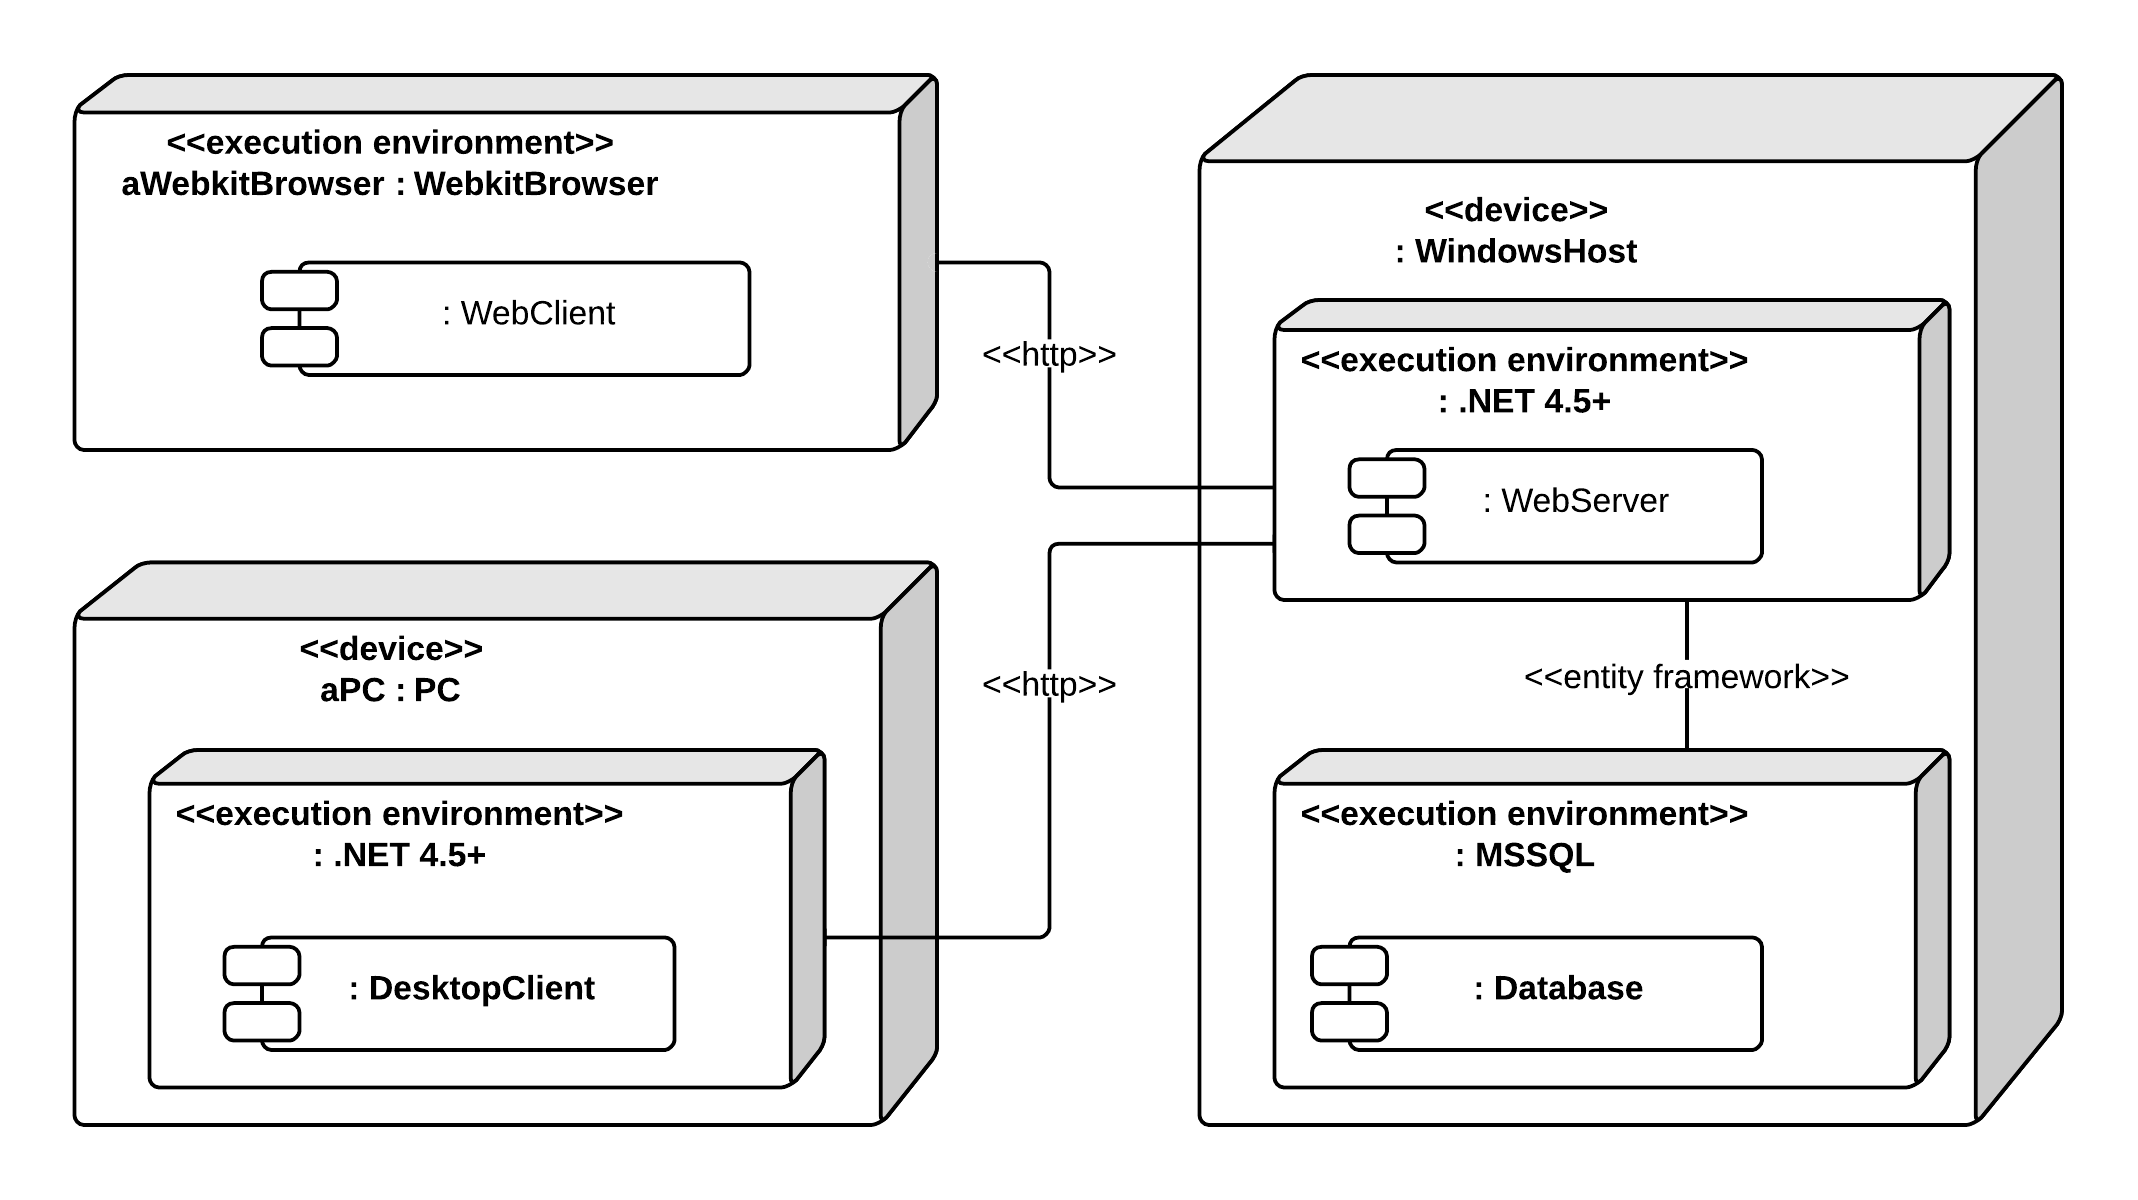
\includegraphics[scale=0.2]{img/SoftwareHardwareMapping.png}
\caption{Software/Hardware Mapping}
\label{fig:SoftwareHardwareMapping}
\end{figure}

\begin{itemize}
\item \textbf{aPC} is the hardware node for our DesktopClient component. The requirement it that it must run on a PC with Windows 7 or 8, utilizing .NET 4.5 or greater
\item \textbf{aWebkitBrowser} is a software environment implementing WebKit 2 or greater, able to execute our WebClient component. There are no requirements to the hardware platform
\item \textbf{WindowsHost} is the server hardware node. On it are two execution environments: .NET 4.5 or greater and MSSQL, required for our WebServer and Database components respectively. The components communicate by entity framework which allows for moving an environment and component to another WindowsHost hardware node.
\end{itemize}

\section{Persistent data management}

\subsection{RDBMS mapping}

\section{Access control and security}
\begin{itemize}
\item Access Control: The idea with this system is to make a IMDb where the users of the system are in control of the content of the available information. The system doesn't operate with different levels of access control. The system has a user who can post information, get information and edit information so that any user have unlimited access to system data.
\item Security: To make a secure system in that sense that messages sent from client to sever and back to client again, is encrypted is out of the scobe for this project.\\
The system do not control who a user is as their is no account with a login and a password in the newest version of FakeIMDb, but the server is prepared for this implementation in a future release.
\end{itemize}

\section{Global software control}
The global control flow is designed as procedure driven control flow with the use of threads to support concurrent users. When a user search for a movie a request is send from the web client and recieved by The WebServer. The WebServer receives the request and start a new thread that create a new RequestDelegater who process the request to Storage. If any, the Webserver receives the answer and send it to the webclient through the Communication Framework.

\section{Identifying services}
We have identified subsystem services for our program. They are shown in the figure below, and more detailed explanations for the services can be found beneath the diagram.

\begin{figure}[H]
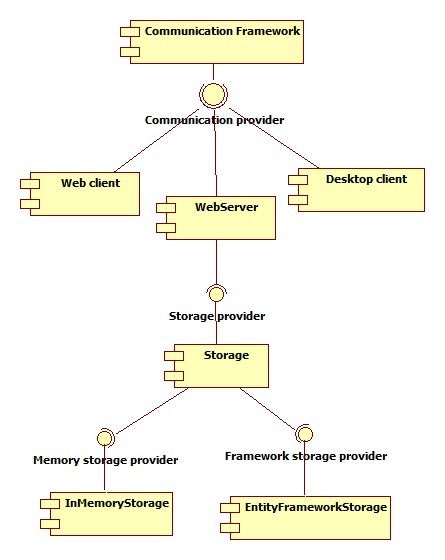
\includegraphics[scale=0.8]{img/SubsystemServices.jpg}
\caption{Software/Hardware Mapping}
\label{fig:Subsystem Services}
\end{figure}


\begin{itemize}
	\item Communication provider, which provides the clients and webserver with access to the communication framework, allowing them to send messages to each other.
	\item Storage provider, which provides the webserver with the methods required to get information / post information to the database.
	\item Framework storage provider, which provides the storage subsystem with the methods needed to store entities in-memory.
	\item Memory storage provider, which provides the storage subsystem with the methods required for storing entities via the entity framework.
\end{itemize}

\section{Boundary conditions}

We have indentified the following boundary conditions, and added them to the list of use cases in the RAD:

\begin{itemize}
	\item Start up and shutdown boundary use cases:
	\begin{itemize}
			\item StartWebServer
			\item ShutdownWebServer
			\item ConfigureWebServer
	\end{itemize}
	\item Exception use cases:
	\begin{itemize}
			\item ServerCrashException
			\item ConnectionLostException
	\end{itemize}
\end{itemize}

\section{Identifying optimization possibilities}